\section{Processing: 45'}

\begin{pyframe}{Simple processing: Goal}
\begin{itemize}
\item Handle gathered data with dicts and zip
\item Find relation between them with scipy
\item Get essential information like standard deviation $\sigma$ and distributions $\delta$
\item Linear correlation: what's that, when can help
distribution and linear correlation.
\end{itemize}
modules: \pymodule{numpy, scipy, scipy.stats.stats, collections, random, time}
\end{pyframe}


\begin{pyframe}{The Chicken Paradox}
\begin{verse}
```According to latest statistics, \\
it appears that you eat one chicken per year: \\
and, if that doesn't fit your budget,\\
you'll fit into statistic anyway,\\
because someone will eat two.'''
\hfill C. A. Salustri
\end{verse}
\end{pyframe}


\iffalse

```Statistics says you'll eat a chicken a year. \\
And even if you can't: statistics doesn't fail! \\
Somebody will surely eat two.''' \\
\fi

\subsection{Distributions}
\begin{pyframe}{Simple processing: Exercise}
Let's gather some data and try to dismantle the chicken paradox
\begin{itemize}
\item Gather 10 seconds of ping output, retrieve a list of RTT
\item Hint: use the sh() function to gather ping output
\item Hint: use zip to put TTL and RTT in two series
\end{itemize}
\end{pyframe}

\iffalse % solution
def ping_rtt():
    """
       goal: slicing data
       goal: using zip to transpose data
    """
    cmd = "ping -c10 www.google.it"
    if 'win' in sys.platform:
        cmd = "ping -n10 www.google.it"

    ping_output = sh(cmd)
    if 'win' in sys.platform:
        ping_output = [ping_output[6::2] for x in ping_output]
    else:
        ping_output = [ping_output[-4:-1:2] for x in ping_output]
    ttl, rtt = zip(*ping_output)
    return map(float, rtt)
\fi


\begin{pyframe}{Distributions: set, defaultdict}
A distribution or $\delta$ shows the frequency of events, like 
how many people ate $x$ chickens ;)
\begin{columns}
\column[t]{.5\textwidth}
\begin{pythoncode}
#Create a simple $\delta$ with
#    set and dict is easy
distro = {x: rtt.count(x) 
  for x in set(rtt)}
  
# We can even use
from collections import defaultdict
distro = defaultdict(int)
for x in rtt:
    distro[x] += 1
    

\end{pythoncode}
\column[t]{.5\textwidth}
\footnotesize
Distributions and Mean are both important!
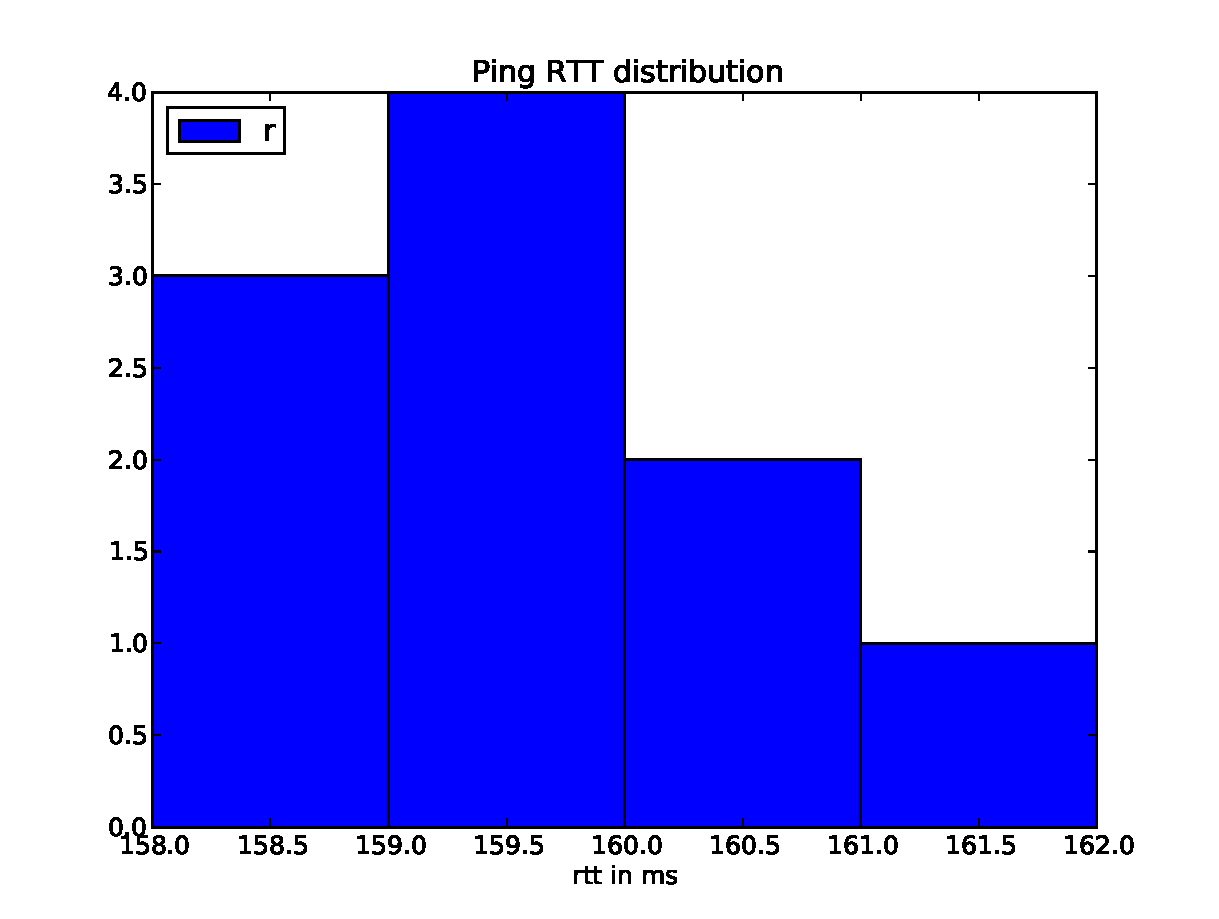
\includegraphics[height=6cm, width=7cm]{ping_distribution.pdf}  
\end{columns}
\end{pyframe}

\subsection{Deviation}
\begin{pyframe}{Standard Deviation: scipy}
\begin{itemize}
\item Standard deviation or $\sigma$ formula is  $\sigma^{2}(X) := \frac{ \sum(x-\bar{x})^{2} }{n} $
\item $\sigma$ tells if $\delta$ is fair or not, and how much the mean ($\bar{x}$) is representative
\end{itemize}
\begin{pythoncode}
from scipy import std, mean
fair = [1, 1] # chickens
unfair = [0, 2] # chickens
assert mean(fair) == mean(unfair)

# Use standard deviation!
std(fair) # 0
std(unfair) # 1
\end{pythoncode}
\end{pyframe}


\begin{pyframe}{Simple processing: scipy}
Check your computed values vs the $\sigma$ returned by ping 
(didn't you notice ping returned it?) 
\begin{pythoncode*}{escapeinside=||}
def ping_stats():
    """goal: remember to convert to numeric / float
       goal: use scipy
       goal: check stdev"""
    from scipy import std, mean # max,min are builtin
    rtt = ping_rtt()
    fmt_s = 'stdev: {}, mean: {}, min: {}, max: {}'
    rtt_std, rtt_mean = |\pyver{std}|(rtt), |\emph{mean}|(ping_rtt)
    rtt_max, rtt_min = max(rtt), min(ping_rtt)
    print(fmt_s.format(rtt_std, rtt_mean, rtt_max, rtt_min))
\end{pythoncode*}
\end{pyframe}

\begin{pyframe}{Time Distributions: Exercise}
\begin{itemize}
\item Parse the \href{https://github.com/ioggstream/python-course/blob/master/python-for-sysadmin/data/maillog}{provided maillog} in ipython using its ! magic and get a 4-hourly email $\delta$
\item Expected output: 
\begin{pythoncode}
time_d = {  # mail sent between
    0: xxx  #  00:00 - 03:59
    4: xxx  #  04:00 - 07:59
    ...
    }
\end{pythoncode}
\end{itemize}
\end{pyframe}
 
\iftrue
\begin{pyframe}{Time Distributions: Exercise Solution}
\begin{pythoncode}
# deliveder emails are like the following
line = "May 14 16:00:04 rpolli postfix/qmgr[11922]: 4AD0C934DA: removed"
def get_slot(ts):
    n = int(ts[:2])
    return n - (n%4)
    
# get the interesting lines
ret = !bzgrep removed maillog
# find the timestamp
ts = ret.fields(2) # 3rd column
hours = [ get_slot(ts)  for x in ts ]
time_d = {x:count(x) for x in set(hours)}
\end{pythoncode}
\end{pyframe}

\fi 

\begin{pyframe}{Size Distributions: Exercise}
\begin{itemize}
\item Parse the provided maillog file and get a size $\delta$
\item Expected output: 
\begin{pythoncode}
size_d = {  # mail size between
    0: xxx  #  0 - 100k
    1: xxx  #  100k - 200k
    ...
    }
\end{pythoncode}
\item Use the $\delta$ to find size\_mean and size\_sigma
\end{itemize}
\end{pyframe}



\begin{pyframe}{Simulating data with $\sigma$ and $\bar{x}$}
We can use  mean and a stdev to simulate data using the gaussian distribution.
This is obviously \emph{just a starting point}.
\begin{pythoncode*}{escapeinside=||}
from random import gauss
# In a mail load generator script we can simulate a
mail_size = int(gauss(mean, sigma_s))

# and use time_d to simulate the load during the day
from time import localtime
hour = localtime().tm_hour
hour = hour - (hour % 4)
mail_per_minute = time_d[hour] / |\pyver{(4 * 60)}| # minutes in 4hours
\end{pythoncode*}
\end{pyframe}

\begin{pyframe}{Plotting distributions}
\begin{pythoncode}
# To plot data...
from matplotlib import pyplot as plt
# and set the interactive mode
plt.ion()

# Plotting an histogram returns a 
distribution = hist(hours)
\end{pythoncode}
\end{pyframe}


\subsection{Correlation}
\begin{pyframe}{Linear Correlation}
\begin{columns}
\column[t]{.6\textwidth}
\begin{pythoncode}
#Let's plot the following 
# datasets
mail_sent = [1, 5, 500, 250, 100, 7]
kB_s = [70, 300, 29000, 12500, 450, 500]

# A scatter plot can suggest relations between data
plt.scatter(mail_sent, kB_s)





\end{pythoncode}
\column[t]{.4\textwidth}
\footnotesize
Correlating Mail and Thruput
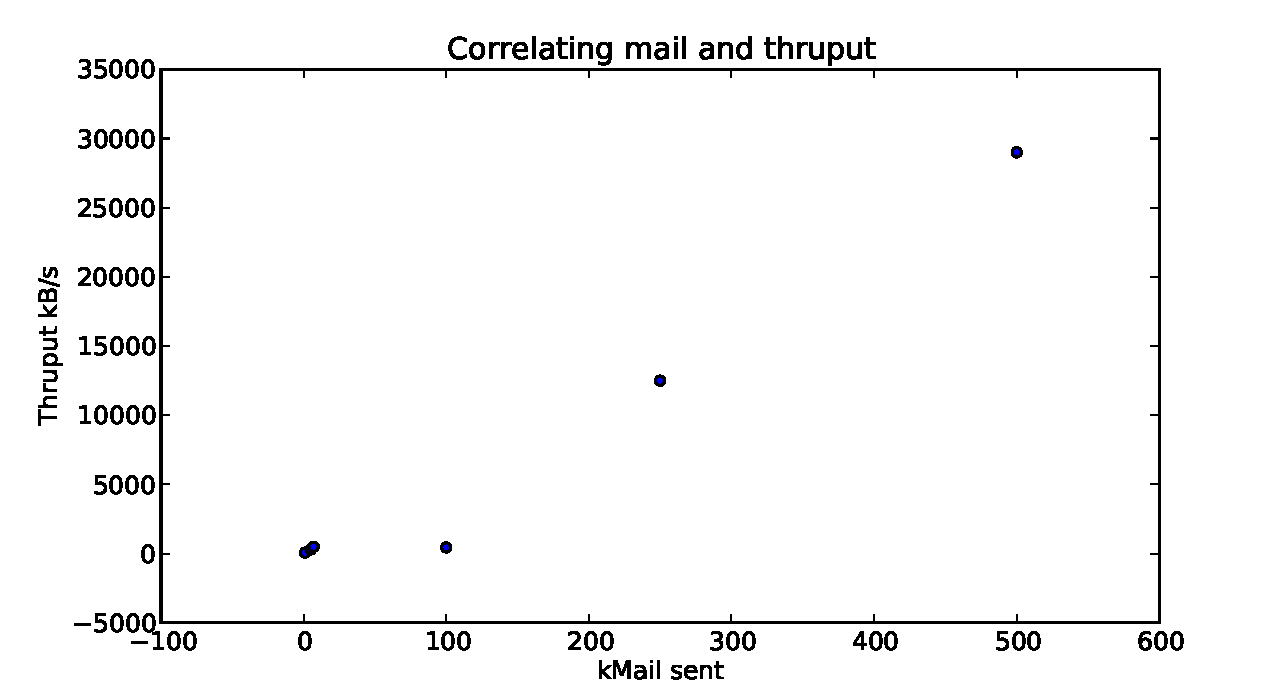
\includegraphics[height=5cm,width=7cm]{scatter_mail.pdf}
\end{columns}
\end{pyframe}


\begin{pyframe}{Linear Correlation}
The Pearson Coefficient is a relation indicator. 
\begin{description}
\item[0]  no relation
\item[1]  direct relation (both dataset increase together)
\item[-1]  inverse relation (one increase as the other decrease) 
\end{description}

\begin{pythoncode}
from scipy.stats.stats import pearsonr
ret = pearsonr(mail_sent, kB_s)
print ret 
>(0.9823, 0.0004)
correlation, probability = ret
\end{pythoncode}
\end{pyframe}

\begin{pyframe}{You \emph{must plot!}}
\LARGE
\begin{center}
PearsonR does not detect non-linear correlation \\
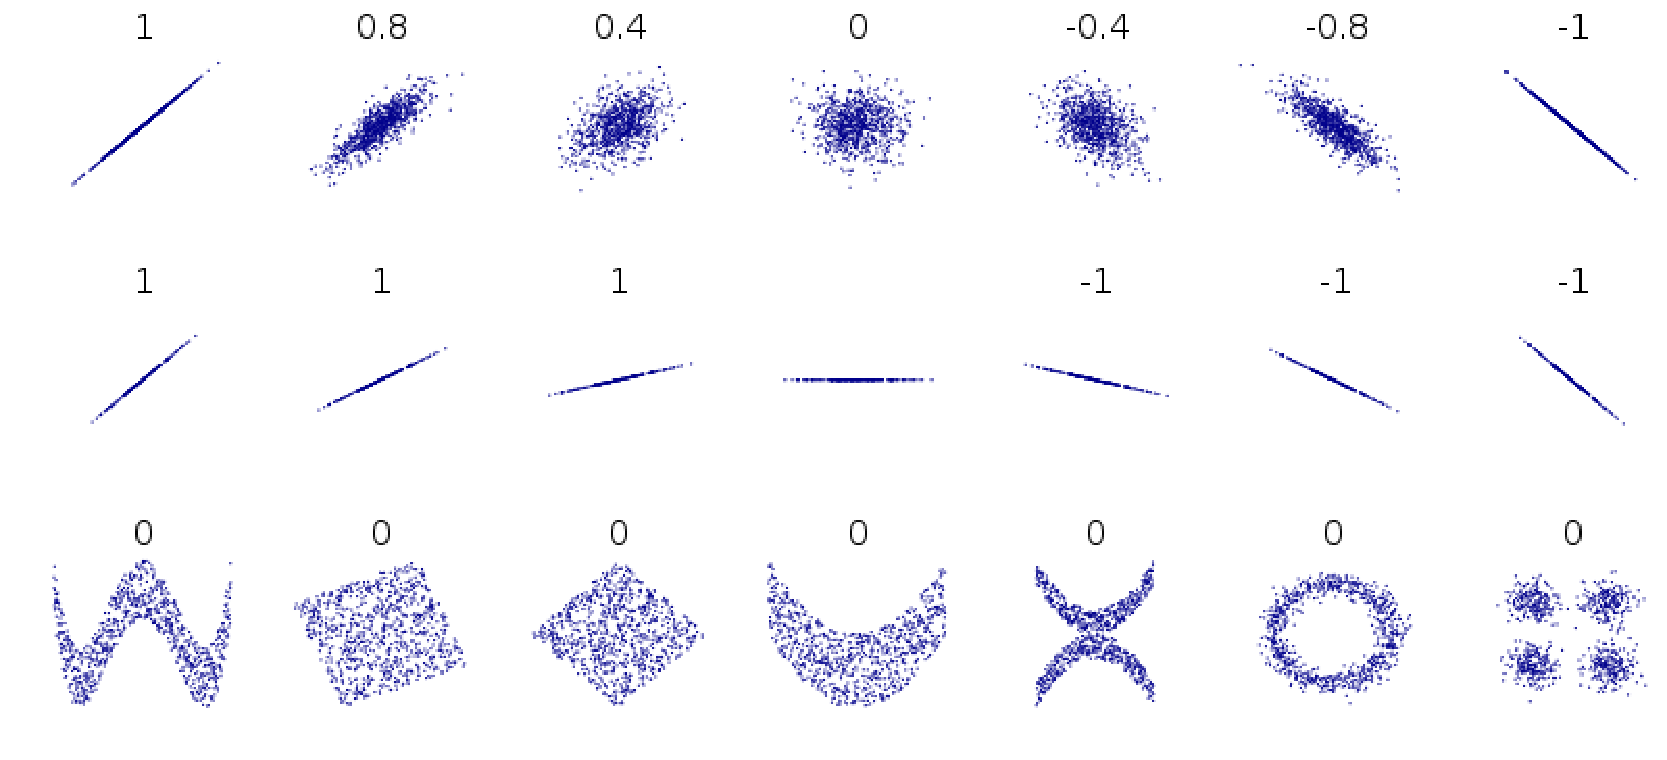
\includegraphics[width=.8\textwidth]{correlation.pdf} \\
\end{center}
\end{pyframe}


\begin{pyframe}{Combinations \dbinom{n}{k}}
\begin{columns}
\column[t]{.7\textwidth}

\begin{pythoncode}
# Given a table with many data series
table = {'cpu_percent': [10, 23, 55, ...],
        'iops': [2132, 3212, 3942, ...],
        'netio': [1.32e+9, 1.45e+9, ...]}

# We can combine all their names with
from itertools import combinations
list(combinations(table,2))
>[('iops', 'netio'), ('iops', 'cpu_percent'), 
  ('netio', 'cpu_percent')]
\end{pythoncode}
\column[t]{.3\textwidth}
\includegraphics{combination_3.pdf}
\end{columns}
\end{pyframe}


\begin{pyframe}{Netfishing correlation}
\begin{pythoncode}
for k1, k2 in combinations(table, 2):
    r_coeff, probability = pearsonr(table[k1], table[k2])
    if r_coeff < 0.5 or probability < 0.1:
        # I'm interested to data outside the above threshold
        continue
    print("linear correlation between {} and {} is {}".format(
        k1, k2, r_coeff))

\end{pythoncode}
\end{pyframe}

\begin{pyframe}{Netfishing correlation II}
\begin{pythoncode}
from matplotlib import pyplot as plt
# create all combined plot
for k1, k2 in combinations(table, 2):
    r_coeff, probability = pearsonr(table[k1], table[k2])
    plt.scatter(table[k1], table[k2])
    # 3 digit precision on title
    plt.title("R={:0.3f} P={:0.3f}".format(r_coeff, probability))
    plt.xtitle(k1) 
    plt.ytitle(k2)
    plt.savefig("{}_{}.png".format(k1, k2))
    plt.close()
\end{pythoncode}
\end{pyframe}


\begin{pyframe}{Mark time with colors}
\begin{pythoncode}
# if our dataseries span 6 time intervals of 4 hours each: color can mark time
from itertools import cycle
colors = cycle(['#ff0000', '#800000', '#00ff00', '#008000','#0000ff', '#000080'])
bucket_size = 4*360      # 4 hours of 10-seconds sampling 
# create all combined plot
for k1, k2 in combinations(table, 2):
    r_coeff, probability = pearsonr(table[k1], table[k2])
    # 3 digit precision on title
    plt.title("R={:0.3f} P={:0.3f}".format(r_coeff, probability))
    plt.xtitle(k1); plt.ytitle(k2)
    for i in range(0, 6):
        t0, t1 = bucket_size*i, bucket_size*(i+1)
        slice_k1, slice_k2 = table[k1][t0:t1], table[k2][t0:t1]
        plt.scatter(slice_k1, slice_k2, next(colors))
    plt.savefig("time_colored_4h_{}_{}.png".format(k1, k2))
    plt.close()
\end{pythoncode}
\end{pyframe}

\section{End}
\begin{pyframe}{That's all folks!}
Thank you for the attention!
\end{pyframe}


